\chapter{Introducción}

Almacenar información es un problema que se lleva desarrollando desde el siglo III a.C, cuando Ptolomeo II fundó la biblioteca de Alejandría que almacenaba todo el saber de la época, entre lo que se incluían obras de teatro, poemas, tratados de medicina y matemáticas. La biblioteca llegó a almacenar hasta 900\,000 ejemplares, pero la información no era valiosa puesto que se guardaba sin ningún tipo de orden, por lo que era imposible explotar la información almacenada de la biblioteca, hasta que Ptolomeo II contactó con Zenodoto, y decidió ordenar los ejemplares de la biblioteca por orden alfabético, pudiendo consultar la información de forma sencilla y explotar el conocimiento que la biblioteca albergaba~\cite{bigdataintroduccion}.\\

En la actualidad, el crecimiento exponencial de internet genera grandes volúmenes de información relevante que es necesario almacenar en grandes centros de datos. Como pasó con Ptolomeo II, es necesrio buscar nuevas formas de almacenar y procesar estos grandes volúmenes de información para generar valor de la información almacenada. Este nuevo paradigma se conoce como Big Data y tiene tres características fundamentales, también llamada la regla de ``las tres uves'': volumen, velocidad y variedad~\cite{bigdataoreilly}.\\
El volumen se refiere a la gran cantidad necesaria de información que se almacena y procesa; ya no se centra en una muestra, sino que se almacena y procesa todo el histórico de datos. La velocidad se refiere a la velocidad que se procesa la información, llegando en algunos casos al tiempo real o ``real-time''. Por último, la variedad se refiere a que la información no llega en un solo formato, sino que hay que procesar varios de ellos, tales como imágenes, documentos, vídeos, audios, etc.\\

Para dar valor a la información almacenada se hace uso de algoritmos de Machine Learning o Aprendizaje Automático, que consiste en diseñar e implementar algoritmos que permitan ``aprender'' a un ordenador a resolver problemas de forma automática, generando soluciones del problema, a partir de unos datos de prueba, y realimentarse para obtener mejores soluciones al problema.\\
El Machine Learning se ha aplicado en muchos casos de éxito como reconocimiento de texto manuscrito~\cite{Murphy:2012:MLP:2380985}, reconocimento facial~\cite{Szeliski:2010:CVA:1941882}, la predicción de mercados financieros~\cite{citeulike:13778368}, ganando al campeón del mundo de Go~\cite{44806}, o mejorando a algunos humanos jugando a juegos clásicos (Figura~\ref{fig:atari}) de Atari~\cite{mnih-dqn-2015}, entre otros.\\

\begin{figure}[tbph!]
\centering
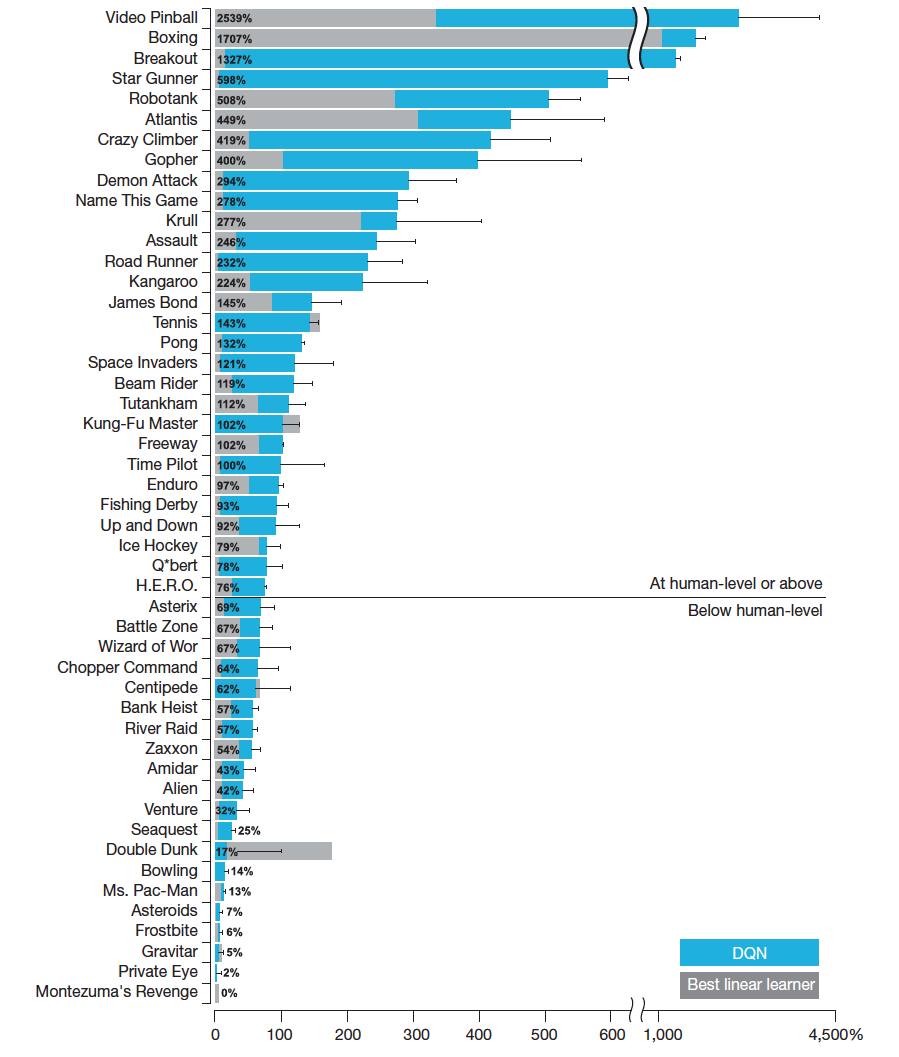
\includegraphics[width=0.7\linewidth]{imagenes/atari.png}
\caption[Juegos de Atari donde un algoritmo de Machine Learning supera a humanos.]{Juegos de Atari donde un algoritmo de Machine Learning supera a humanos. Fuente:~\cite{mnih-dqn-2015}}

\label{fig:atari}
\end{figure}

En la memoria nos centraremos en el Machine Learning y pondremos énfasis en los tipos que existen y qué algoritmos hay disponibles. Además, describiremos un nuevo método basado en teoría de grafos, y lo compararemos con otros algoritmos clásicos, desarrollando una aplicación que permita analizar conjuntos de datos y comparar entre distintos algoritmos. Por último, usaremos la aplicación para analizar un conjunto de datos.\\

El proyecto tiene los siguientes objetivos:

\begin{enumerate}
\item Introducir qué es el Machine Learning, qué tipos de Machine Learning existen según el tipo de aprendizaje, qué problemas se pueden resolver aplicándolo y familiarizarse con algunos de los algoritmos clásicos.

\item Introducir los conceptos básicos de teoría de grafos, como algunas medidas de redes complejas.

\item Dar a conocer nuevos algoritmos de Machine Learning basados en teoría de grafos, conocidos como redes parenclíticas.

\item Desarrollar una aplicación que automatice el proceso del aprendizaje según distintos algoritmos de Machine Learning (clásicos y basados en teoría de grafos).

\item Analizar una base de datos y comparar los resultados de los distintos algoritmos de Machine Learning.
\end{enumerate}

La memoria está estructurada de la siguiente forma:\\

En el Capítulo~\ref{cap:ml} se introduce el concepto de Machine Learning, qué tipos hay según el aprendizaje y qué tareas permite resolver, así como algunos de los algoritmos existentes según el tipo de aprendizaje.\\

En el Capítulo~\ref{cap:redes_parencliticas}, se introducen brevemente la teoría de grafos, así como un nuevo algoritmo de Machine Learning basado en grafos, las redes parenclíticas.\\

En el Capítulo~\ref{cap:diseño}, se presenta el desarrollo de una aplicación que permita analizar una base de datos utilizando distintos algoritmos de Machine Learning, y compararlos entre ellos.\\

En el Capítulo~\ref{cap:aplicacion}, se analiza una base de datos usando distintos algoritmos de Machine Learning, y una comparación entre ellos.\\

En el Capítulo~\ref{cap:conclusiones}, se presentan las conclusiones y el trabajo futuro. 


%En la actualidad los seres humanos somos unos grandes generadores de datos: al visitar una página web nuestros hábitos de navegación (tipo de ordenador utilizado, navegador, país, hora, etc) quedan almacenados en los servidores de la página web; al realizar una transacción bancaria, nuestro banco guarda datos acerca del cajero utilizado, a qué hora se ha realizado, desde qué país, etc. Éstos son algunos de los lugares donde son recogidos nuestros datos, aunque existen infinidad de ellos.\\

%El objetivo no es almacenar únicamente los datos, sino obtener valor de ellos: en el caso de la página web, se usarán los datos para obtener anuncios o compras (si es una tienda) personalizados, o bloquear tráfico, en caso de que se estuviera produciendo un ataque hacia la página web. En el caso del banco, podría usar los datos para para ofrecer productos personalizados o bloquear transacciones que no se adecuen al comportamiento de un usuario.\\

%Para lograr ésto, se necesitan algoritmos que permitan a los ordenadores ``aprender'' a partir de un conjunto de datos de entrada, para posteriormente inferir sobre nuevos datos. De ésto se encarga el Machine Learning o Aprendizaje Automático.\\

%A lo largo de la memoria veremos qué es el machine learning, qué tipos hay según el tipo de aprendizaje y qué problemas se pueden resolver usándolo, y los algoritmos de machine learning más utilizados.\\

%También veremos otros algoritmos más novedosos: las redes parenclíticas, basadas en teoría de grafos.\\

%Con todo ésto, desarrollaremos una aplicación web para analizar distintos conjuntos de datos usando algoritmos clásicos de machine learning y redes parenclíticas y poder comparar entre ambos algoritmos.\\

%Por último, utilizaremos la aplicación para la detección de tumores en cáncer de mama.  